%Cody Lewis, Luke De Ruyter, 2012
%Visit anzhelka.com for all the latest
%
% CTRL+SPACE to switch panes in Texmaker
%
% Note: blank lines indicate a new paragraph
% Note: \left( and \right) cannot break lines.

% TODO: Additional material
% --- Section 2.1 still needs more content

% Needs approval and over sight from Cody :)


\documentclass[english]{article}

% Packages that are being used.
\usepackage{amsmath}
\usepackage{longtable}
\usepackage{color}
%\usepackage{verbatim} % used to display code
\usepackage{listings}
\usepackage{graphicx}
\usepackage{subfigure}
\usepackage{indentfirst}
\usepackage{fancyhdr} % Fancy Header
\usepackage{rotating} % To make vertical text in tables
\usepackage[normalem]{ulem} %for strikethroughs

\usepackage{enumerate} % For letter/number list

%\usepackage{babel}

%\usepackage{hyperref} %Must be at the end of use package but before "other settings". Used to make links of all references.




\numberwithin{equation}{section} %change the numbering to have something like 1.1 and 3.15, etc.
%Format of macro:
%\newcommand{\NAME}[ARGUMENT NUMBER (OPTIONAL)]{ stuff to include, arguments denoted #1, #2, etc. }
\newcommand{\vect}[1]{\boldsymbol{#1^2}}
\newcommand{\bigvect}[3]{\boldsymbol{#1^#2^#3}}
\newcommand{\bs}[1]{\boldsymbol{#1}}

%\addto{\captionsenglish}{\renewcommand*{\appendixname}{MyAppx}}

\definecolor{lightlightgray}{gray}{0.9}

\graphicspath{{../tests/}{../figures/}{../extra/}{../figures/editorial/}} %\graphicspath{{path/one/}{path/two/}{path/three/}}

\fancyhead[RO,RE]{\textit{Page \thepage}}
\fancyhead[CO,CE]{}
\fancyhead[LO,LE]{\textit{Software Requirements Specification for Anzhelka}}
\fancyfoot[CO,CE]{ \thepage \\ 
\includegraphics[width=2cm]{../extra/pheonix_small.png}}
\pagestyle{fancy}

\setcounter{tocdepth}{1} %display only sections in table of contents

\begin{document}

\pagenumbering{roman}

\lstset{
%language=C,                             % Code langugage
basicstyle=\ttfamily,                   % Code font, Examples: \footnotesize, \ttfamily
keywordstyle=\color{OliveGreen},        % Keywords font ('*' = uppercase)
commentstyle=\color{gray},              % Comments font
%numbers=left,                           % Line nums position
%numberstyle=\tiny,                      % Line-numbers fonts
%stepnumber=1,                           % Step between two line-numbers
%numbersep=5pt,                          % How far are line-numbers from code
backgroundcolor=\color{lightlightgray}, % Choose background color
frame=none,                             % A frame around the code
tabsize=4,                              % Default tab size
captionpos=b,                           % Caption-position = bottom
breaklines=true,                        % Automatic line breaking?
breakatwhitespace=false,                % Automatic breaks only at whitespace?
showspaces=false,                       % Dont make spaces visible
showtabs=false,                         % Dont make tabls visible
%columns=flexible,                       % Column format
%morekeywords={__global__, __device__},  % CUDA specific keywords
}







%\\ Version 1.0 approved \\ Prepared by Luke De Ruyter, Cody Lewis \\ University of California, Riverside \\ \date{\today}
\title{\begin{flushright}\textbf{
\rule{\textwidth}{3 pt} \\
\bigskip \bigskip
\Huge Software/Hardware \\ 
Requirements Specification \\ 
\bigskip \LARGE for \\ \bigskip
\Huge Anzhelka \\
\bigskip \bigskip \bigskip
\large Version 1.0 approved \\
\bigskip \bigskip \bigskip
Prepared by \\ Luke De Ruyter \\Cody Lewis \\
\bigskip \bigskip \bigskip
University of California, Riverside \\
\bigskip \bigskip \bigskip
\today
}\end{flushright}}
%\author{Cody Lewis \\ \texttt{srlm@anzhelka.com} \and Luke De Ruyter \\ \texttt{ilukester@anzhelka.com} }
%\date{\today}
\date{}
\author{}
\maketitle 
\newpage

%\begin{center}
\includegraphics[scale=.24]{tribal_phoenix.jpg}\end{center}

%% TOC TOC TOC TOC TOC TOC TOC TOC TOC TOC TOC TOC
\renewcommand{\contentsname}{Table of Contents}
\tableofcontents
%\addcontentsline{toc}{section}{Table of Contents}
%% TOC TOC TOC TOC TOC TOC TOC TOC TOC TOC TOC TOC


%% REV REV REV REV REV REV REV REV REV REV REV REV REV
\section*{Revisions}
Current project status and files can be found at
\begin{center}
 \textbf{blog.anzhelka.com} \\
 \textbf{code.anzhelka.com} \\
\end{center}

\begin{longtable}{l | l | p{5cm} | l}
\hline
\textbf{Version} & \textbf{Date} & \textbf{Changes} & \textbf{Commiter}\\
\hline
0.01	& April 30, 2012 & Initial layout of file was created. 	& Cody \\
\hline
0.02	& May 4, 2012 & Purpose, Audience, Scope, Perspective, Functions, and Users was populated. & Cody, Luke \\
\hline
\end{longtable}

%% REV REV REV REV REV REV REV REV REV REV REV REV REV


\newpage
\pagenumbering{arabic}


%% S1 S1 S1 S1 S1 S1 S1 S1 S1 S1 S1 S1 S1 S1 S1 S1 S1 S1 S1 S1  

%% S1 S1 S1 S1 S1 S1 S1 S1 S1 S1 S1 S1 S1 S1 S1 S1 S1 S1 S1 S1  

%% S1 S1 S1 S1 S1 S1 S1 S1 S1 S1 S1 S1 S1 S1 S1 S1 S1 S1 S1 S1  
\section{Introduction}
\subsection{Purpose}
Anzhelka is a complete system intended for autonomous quadrotor flight. Included as a part of Anzhelka is both hardware and software. This includes the quadrotor frame, control electronics, ground station software, and the complete system documentation. Anzhelka is completely open source, and all project files are available for download. You can find in this document any instructions necessary for understanding the functionality of Anzhelka components. This includes hardware and software interfaces, features, and system requirements.
\subsection{Document Conventions}
\subsection{Intended Audience and Reading Suggestions}
This document is written for Anzhelka developers. This document is intended to refine development direction, and to bring new developers up to speed. For this document, developers include software writers, hardware designers, and system testers. When the word "you" is written, it is referring to the developer who is reading this document. When the words "the user" is written, it is referring to the end user of the Anzhelka platform.

You should read this document based on your background with Anzhelka. Current developers can find the appropriate section to read. New developers should read the introduction, overall description, and system features sections. If you are a non-developer for this project, and don't intend to ever become one, you should avoid this document. Look on the Anzhelka website for something more appropriate to your needs.


\subsection{Product Scope}
Anzhelka consists of four main components: a quadrotor hardware frame, custom quadrotor software, ground station software, and detailed documentation via the Anzhelka website. Even without a degree in control systems, you can use Anzhelka components to make an autonomous quadrotor system. By using these components you can customize the functionality of the system to suit your needs, or use them directly to perform predefined commands.


\subsection{References}

\newpage
\section{Overall Description}
\subsection{Product Perspective}

\begin{figure}[h!]
  \centering
	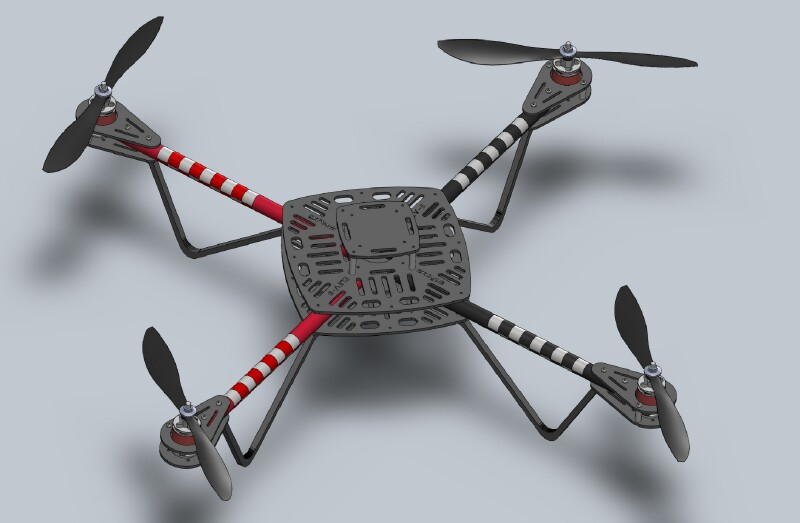
\includegraphics[scale=.6]{elev_8_rendering.JPG}
  \caption{This is an artistic rendering of the frame used for Anzhelka.}
\end{figure}  
Anzhelka is a platform for experimentation in aerial robotics. It is an independent project designed from the ground up. We are taking an existing open hardware frame as our base hardware platform. We have chosen to build on top of this hardware because of its expandability and its durability. We have designed a custom control board that will be able to run all of Anzhelka's software and house all the necessary components.\\
%
%
%\textit{<Describe the context and origin of the product being specified in this SPECIFICATION. For example, state whether this product is a follow-on member of a product family, a replacement for certain existing systems, or a new, self-contained product. If the SPECIFICATION defines a component of a larger system, relate the requirements of the larger system to the functionality of this software or hardware and identify interfaces between the two. A simple diagram that shows the major components of the overall system, subsystem interconnections, and external interfaces can be helpful.>}


\subsection{Product Functions}
Anzhelka is designed to be programmatically controllable in a number of different aspects. The quadrotor can receive commands to set any of it's internal registers, which then affect the flight of the quadrotor. In addition, the quadrotor has a command interpreter that is able to read command sequences from onboard memory. With these commands, the user can control a number of quadrotor functions including attitude and position.

Anzhelka is equipped with a Parallax Propeller multicore processor. The quadrotor has two separate batteries. One battery provides power for the motors and servos; the other battery powers the electronics. The electronic hardware is designed with expandability in mind. The motors and servos have voltage and current monitoring. The Anzhelka system is designed to allow for the easy attachment of additional electronics.

\subsection{User Classes and Characteristics}
%\textit{<Identify the various user classes that you anticipate will use this product. User classes may be differentiated based on frequency of use, subset of product functions used, technical expertise, security or privilege levels, educational level, or experience. Describe the pertinent characteristics of each user class. Certain requirements may pertain only to certain user classes. Distinguish the most important user classes for this product from those who are less important to satisfy.>}

\subsubsection{User Example: Jason}

\begin{figure}[h!]
  \centering
	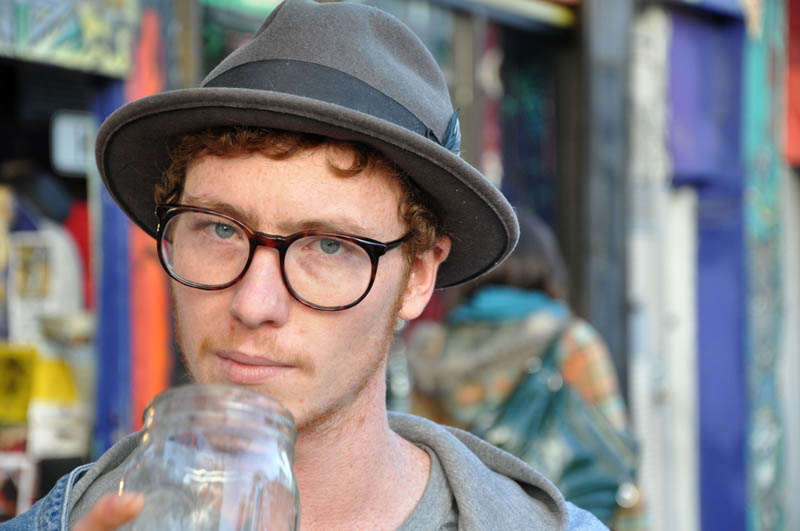
\includegraphics[width=3in]{hipster1.jpg}
  \caption{Jason Lariart}
\end{figure}

\textbf{ Age:} 28

\textbf{ Education:} Some College

\textbf{ Marital Status:} Open

\textbf{ Occupation:} Videographer

\textbf{ Hobbies:} Photography, Videography, Art, Protesting

\textbf{About Jason:} He is an avid videographer and likes to push the limits of his skills, crew, and equipment. He likes to take pictures and videos of things that not just any ordinary person can do. Jason is currently an amateur photographer, but wants to make a professional career out of his work.
\\

\textbf{Scenario:} Jason is preparing for a remote video shoot and realized that he won't be able to get his aerial shot because a helicopter is out of his budget. Jason told the client that he was going to have to spend more money if wanted to get the aerial shot as planned. The client was upset to hear about this and had no choice but to drop the scene from the shoot. %  programmed it so he was able to acchieve the same effect he was looking for while staying in the budget.

\newpage
\subsubsection{User Example: Dan}

\begin{figure}[h!]
  \centering
	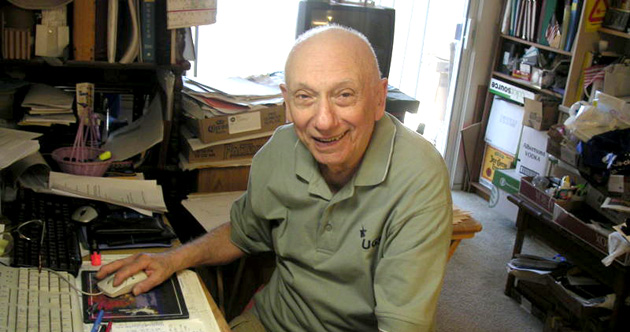
\includegraphics[width=3in]{oldgradstudent.jpg}
  \caption{Dan Knuth}
\end{figure}
\textbf{ Age:} 82

\textbf{ Education:} Doctorate in Mathematics

\textbf{ Marital Status:} Widowed

\textbf{ Occupation:} Software Developer

\textbf{ Hobbies:} Open source programming, online forum posting, sitting

\textbf{About Dan:} Dan works on open source systems. He has literally been around since the begining, and he remembers the days of punch card programming. Throughout his career he has been a strong supporter of making computer science more accessible, and his work in the open source field is both notable and well respected.
\\
\textbf{Scenario:} Dan wants to spend more time focusing on his hobbies, but he doesn't have much time left and he needs to eliminate routine activities. Dan wants to develop a robot to automatically pick up his medicine from the pharmacy and carry it to him. This robot needs to be able to fly, and to be user programmable. Dan has lots of experience in working with software, so it's ok if the product is a bit rough and requires the use of a command line. Dan would be particularly appreciative if the instructions could be programmed in by a series of toggle switches and incandescent lights.

\subsection{Operating Environment}
\subsection{Design and Implementation Constraints}
\subsection{User Documentation}
\subsection{Assumptions and Dependencies}

\newpage
\section{External Interface Requirements}
\subsection{User Interfaces}
\subsection{Hardware Interfaces}
\subsection{Software or Hardware Interfaces}
\subsection{Communications Interfaces}

\newpage
\section{System Features}


\subsection{Attitude Control}
\subsubsection{Description and Priority}
\subsubsection{Stimulus/Response Sequences}

\begin{longtable}{p{3cm} | p{10cm}}
\hline
\textbf{Stimulus} & \textbf{Response}\\
\hline
1. Hit By High Velocity Paintballs &
\begin{enumerate}[(a)]\itemsep1pt %for small alpha-characters within brackets.
\item Paintball hits, creates sudden attitude disturbance
\item Quadrotor loses altitude, increase in attitude error
\item Attittude mathematical control loop gains change to compensate
\item Quadrotor adjusts motor speed based on control loop result
\item Quadrotor achieves desired attitude
\end{enumerate}
\\ 
\hline
\end{longtable}



\subsubsection{Functional Requirements}
\bigskip
\subsection{Altitude Control}
\subsubsection{Description and Priority}
\subsubsection{Stimulus/Response Sequences}

\begin{longtable}{p{3cm} | p{10cm}}
\hline
\textbf{Stimulus} & \textbf{Response}\\
\hline
1. Altitude drops by 5cm &
\begin{enumerate}[(a)]\itemsep1pt %for small alpha-characters within brackets.
\item Quadrotor loses 5cm in altitude
\item Altitude sensor on the Quadrotor triggers an alarm within controll loop
\item Altittude mathematical control loop gains change to compensate
\item Quadrotor adjusts motor speed based on control loop result
\item Quadrotor achieves desired altitude
\end{enumerate}
\\ 
\hline
\end{longtable}



\subsubsection{Functional Requirements}
\bigskip
\subsection{Highly Manueverable}
\subsubsection{Description and Priority}
\subsubsection{Stimulus/Response Sequences}

\begin{longtable}{p{3cm} | p{10cm}}
\hline
\textbf{Stimulus} & \textbf{Response}\\
\hline
1. Quadrotor is programmed to do a barrel roll &
\begin{enumerate}[(a)]\itemsep1pt %for small alpha-characters within brackets.
\item Quadrotor is triggered to preform a barrel roll
\item Current IMU and Altitude readings are stored
\item The trajectory math is calculated by the barrel roll function
\item Motors are changed to the desired speeds calculated by the math
\item The Quadrotor is then returned back to its starting Attitude and Alitude readings
\end{enumerate}
\\ 
\hline
\end{longtable}



\subsubsection{Functional Requirements}
\bigskip
\subsection{User Programmable}
\subsubsection{Description and Priority}
\subsubsection{Stimulus/Response Sequences}

\begin{longtable}{p{3cm} | p{10cm}}
\hline
\textbf{Stimulus} & \textbf{Response}\\
\hline
1. User wants to program the Quadrotor with a new trajectory plan &
\begin{enumerate}[(a)]\itemsep1pt %for small alpha-characters within brackets.
\item User plugs the SD card into their computer
\item User launches the programming software
\item Trajectories are entered into the software
\item When the user is ready they can press the "Write to SD Card" Button
\end{enumerate}
\\ 
\hline
\end{longtable}



\subsubsection{Functional Requirements}
\bigskip
\subsection{Modularized} 
\subsubsection{Description and Priority}
\subsubsection{Stimulus/Response Sequences}

\begin{longtable}{p{3cm} | p{10cm}}
\hline
\textbf{Stimulus} & \textbf{Response}\\
\hline
1. The user wants to fix one of the motor booms &
\begin{enumerate}[(a)]\itemsep1pt %for small alpha-characters within brackets.
\item The user can dissasemble the parts of the frame that were broken
\item The parts can be reassembled together with new or used parts
\end{enumerate}
\\ 
\hline
\end{longtable}



\subsubsection{Functional Requirements}
\bigskip
\subsection{Ground Station}
\subsubsection{Description and Priority}
\subsubsection{Stimulus/Response Sequences}

\begin{longtable}{p{3cm} | p{10cm}}
\hline
\textbf{Stimulus} & \textbf{Response}\\
\hline
1. The user wants to get data from the quadrotor in real time &
\begin{enumerate}[(a)]\itemsep1pt %for small alpha-characters within brackets.
\item The user would turn on the ground station
\item Next they would locate the switch on the control board labeled wireless
\item Toggle the switch to the ON position
\item Connect the ground station to your computer
\item Launch the ground station software 
\end{enumerate}
\\ 
\hline
\end{longtable}



\subsubsection{Functional Requirements}
\bigskip
\subsection{Waypoint Control}
\subsubsection{Description and Priority}
\subsubsection{Stimulus/Response Sequences}

\begin{longtable}{p{3cm} | p{10cm}}
\hline
\textbf{Stimulus} & \textbf{Response}\\
\hline
1. The user wants to control the quadrotor to fly in an contiunous patern &
\begin{enumerate}[(a)]\itemsep1pt %for small alpha-characters within brackets.
\item While the user is using the programming software select the waypoint tab
\item The user then selects the waypoint patern
\item Once that is complete the user can select the contuinous run box
\end{enumerate}
\\ 
\hline
\end{longtable}



\subsubsection{Functional Requirements}
\bigskip
\subsection{Object Tracking}
\subsubsection{Description and Priority}
\subsubsection{Stimulus/Response Sequences}

\begin{longtable}{p{3cm} | p{10cm}}
\hline
\textbf{Stimulus} & \textbf{Response}\\
\hline
1. The user wants to enable the object avoidance software &
\begin{enumerate}[(a)]\itemsep1pt %for small alpha-characters within brackets.
\item The user needs to locate the Object Avoidance switch on the control board
\item The user would then need to toggle the switch into the ON position
\end{enumerate}
\\ 
\hline
\end{longtable}



\subsubsection{Functional Requirements}
\bigskip
\subsection{Intuitive User Control}
\subsubsection{Description and Priority}
\subsubsection{Stimulus/Response Sequences}

\begin{longtable}{p{3cm} | p{10cm}}
\hline
\textbf{Stimulus} & \textbf{Response}\\
\hline
1. The user wants to control the quadrotor manually/ without programming flight data &
\begin{enumerate}[(a)]\itemsep1pt %for small alpha-characters within brackets.
\item The user needs to locate the manual flight switch on the control board
\item The user would then need to toggle the switch into the user position
\item The user would now use the remote control to fly the quadrotor
\end{enumerate}
\\ 
\hline
\end{longtable}



\subsubsection{Functional Requirements}
\bigskip
\subsection{Comprehensive Datalogging}
\subsubsection{Description and Priority}
\subsubsection{Stimulus/Response Sequences}

\begin{longtable}{p{3cm} | p{10cm}}
\hline
\textbf{Stimulus} & \textbf{Response}\\
\hline
1. The user wishes to log all flight data &
\begin{enumerate}[(a)]\itemsep1pt %for small alpha-characters within brackets.
\item The user needs to locate the logging switch on the control board
\item The user would then need to toggle the switch into the logging position
\item Recording begins once flight has been initiated
\end{enumerate}
\\ 
\hline
\end{longtable}



\subsubsection{Functional Requirements}
\bigskip
\subsection{Open Community Support}
\subsubsection{Description and Priority}
\subsubsection{Stimulus/Response Sequences}

\begin{longtable}{p{3cm} | p{10cm}}
\hline
\textbf{Stimulus} & \textbf{Response}\\
\hline
1. The user has a problem with troubleshooting a problem that they are having. &
\begin{enumerate}[(a)]\itemsep1pt %for small alpha-characters within brackets.
\item The user can browse to our forum website forums.anzhelka.com
\item They can then select the Troubleshooting directory
\item They would then need to log in or create a new account
\item Click on the "Create a new Thread" button
\item They would then need to come up with a descriptive title for their problem.
\item Now the would need to explain in great detail what their problems are and what they have tried to do to solve it.
\item The user should check back regularly to see if anyone has commented on their thread.
\end{enumerate}
\\ 
\hline
\end{longtable}



\subsubsection{Functional Requirements}



\subsection{System Feature 2 (and so on)}




\newpage
\section{Other Nonfunctional Requirements}
\subsection{Performance Requirements}
\subsection{Safety Requirements}
\subsection{Security Requirements}
\subsection{Software or Hardware Quality Attributes}
\subsection{Business Rules}

\newpage
\section{Other Requirements}
\appendix
%\gdef\thesection{Appendix \Alph{section}:}
\section{Glossary}
\section{Analysis Models}
\section{To Be Determined List}


\end{document}
